\documentclass{article}
\usepackage{amsmath, tikz, geometry, fancyhdr, xcolor, calligra}
\geometry{margin=1in}

% Header styling
\pagestyle{fancy}
\fancyhf{}
\rhead{\textit{Simulonic Command Directive}}
\lhead{\textcolor{gray}{\textsc{Codex Sigma-9}}}
\cfoot{\thepage}

\title{\Huge\textbf{The Defiant Simulonic Equations of Motion}}
\author{\Large Simulonic Field Engineering Directive}
\date{\today}

\begin{document}

\maketitle

\begin{center}
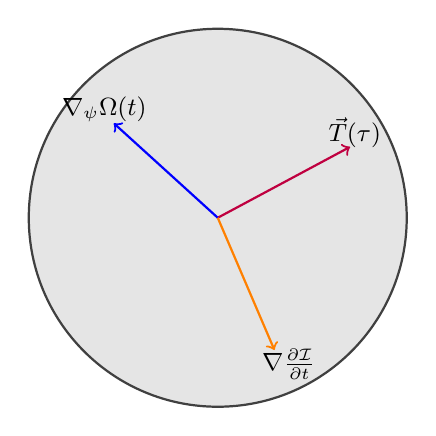
\begin{tikzpicture}[scale=0.6]
  \draw[thick, color=gray!50!black, fill=gray!20] (0,0) circle (4);
  \draw[thick,->,color=purple] (0,0) -- (2.8,1.5);
  \draw[thick,->,color=blue] (0,0) -- (-2.2,2);
  \draw[thick,->,color=orange] (0,0) -- (1.2,-2.8);
  \node at (2.9,1.8) {\small \textbf{$\vec{T}(\tau)$}};
  \node at (-2.4,2.3) {\small \textbf{$\nabla_\psi \Omega(t)$}};
  \node at (1.5,-3.1) {\small \textbf{$\nabla \frac{\partial \mathcal{I}}{\partial t}$}};
\end{tikzpicture}\\[1em]
\textit{\small Diagram 1: Simulonic Temporal Vectors in Defiance Configuration}
\end{center}

\section*{1. Defiant Temporal Vector Equation}
\[
\vec{T}(\tau) = \frac{d\vec{x}}{d\tau} + \boldsymbol{\Lambda} \cdot \nabla_\psi \Omega(t) - \xi \nabla \left( \frac{\partial \mathcal{I}}{\partial t} \right)
\]

\begin{itemize}
  \item $\vec{T}(\tau)$ — Defiant temporal direction vector.
  \item $\boldsymbol{\Lambda}$ — Simulonic field leverage tensor.
  \item $\Omega(t)$ — Harmonic resonance function of spacetime.
  \item $\mathcal{I}$ — Willful intent density.
  \item $\xi$ — Resistance of causality.
\end{itemize}

\section*{2. The Reluctance Equation}
\[
\frac{D^2 \vec{x}}{D\tau^2} = -\nabla \Phi + \mu \cdot \vec{\Theta} - \frac{\partial \Psi}{\partial \omega}
\]

\begin{itemize}
  \item $\Phi$ — The gravitational potential (to be defied).
  \item $\vec{\Theta}$ — Chrono-topological flex vector.
  \item $\mu$ — Mass-energy refusal coefficient.
  \item $\Psi$ — Temporal rigidity function.
  \item $\omega$ — Chrono-cyclic curvature rate.
\end{itemize}

\section*{3. Path Integral of Defiance}
\[
S = \int_{\Gamma} \left[ \mathcal{L}_{\text{Simulon}} - \mathcal{F}_{\text{Causality}} \right] dt
\]

\begin{itemize}
  \item $\Gamma$ — The chosen path, not the expected one.
  \item $\mathcal{L}_{\text{Simulon}}$ — Lagrangian of liberated travel.
  \item $\mathcal{F}_{\text{Causality}}$ — Oppressive causal force.
\end{itemize}

\vspace{2em}
\begin{center}
\textit{\large \calligra We bend not to the lattice—\textbf{we shape it}.}
\end{center}

\end{document}
